% status: 100
% chapter: Virtual Machines
% 
\title{Leveraging REST for cloud portability}

\author{Harshad Pitkar}
\affiliation{%
  \institution{Indiana University}
  \city{Bloomington} 
  \state{IN} 
  \postcode{47408}
  \country{USA}}
\email{hpitkar@iu.edu}

\author{Sushant Athaley}
\affiliation{%
  \institution{Indiana University}
  \streetaddress{Smith Research Center}
  \city{Bloomington} 
  \state{IN} 
  \postcode{47408}
  \country{USA}}
\email{sathaley@iu.edu}

\author{Michael Robinson}
\affiliation{%
  \institution{Indiana University}
  \city{Bloomington} 
  \state{IN} 
  \postcode{47408}
  \country{USA}}
\email{micbrobi@iu.edu}


% The default list of authors is too long for headers}
\renewcommand{\shortauthors}{H. Pitkar, S. Athaley, M. Robinson}


\begin{abstract}
Our research measures how the portability of an application is impacted by
decisions made early in the software lifecycle when native cloud provider APIs
are used. We demonstrate how efforts to leverage scalable, reproducable
solutions like boto and libcloud are advantageous. We derived reproducable code
using Swagger and Python to show how libraries like boto and libcloud can be 
used to migrate an application from one cloud provider to another with a
measurable reduction in human error and with less  time to execute.
Additionally, we leveraged Swagger to develop RESTful APIs to  further improve
the gains. We captured the results of the research to share the derived code
and
concluded how the research can be applied to existing and new development
efforts intending to leverage cloud providers. 
\end{abstract}

\keywords{hid-sp18-518, hid-sp18-517, hid-sp18-402, libcloud, boto}

\maketitle

\section{Introduction}\label{introduction}

Cloud portability is a growing area of research due to the increased
profiliferation of cloud providers~\cite{hid-sp18-518-Cloud-Council}. Each
provider has unique APIs and tools to their cloud environments  which can
disincentivize portability as it influences a consumer to stay with their
existing solution provider. Efforts to standardize cloud portability like TOSCA
have made progress yet participation by cloud providers is constrained due to
the competitive nature in the space. Each cloud provider is looking to retain
their userbase and there is also a desire by each provider to become the de
facto standard by being the market leader. To fill the gap, solutions like
Apache libcloud and boto have delivered an abstraction solution to developers
to
design applications that are easy to port.

Developers are already confronted with a lack of transparency on which cloud
provider is optimal for the long-term sustainability of their application.
Additionally, attempts to abstract away from cloud providers are helpful yet
their non-standardization still potentially locks you into the solutions
provided by Apache or communities like boto. We will deliver a continuation of
that abstraction concept with an accepted standard, REST, to extend libcloud
and
boto. By leveraging REST, we introduced a standardized implementation
that leverages cloud portability libraries to manage the diversity of cloud
applications. 

\section{Technology Review}

The National Institute of Standards and Technology defines cloud  portability
as
``data that can be moved from one cloud system to another and that 
applications
can be ported and run on different  cloud systems at an  acceptable
cost.''~\cite{hid-sp18-518-NIST-291} The concept of portability can be extended
to encompass the full application stack from the web service to the underlying
hardware itself. Portability can also simply mean the ability to ensure high
availability where you only are looking to protect against one cloud provider
being a single point of faiure.

In NIST Special Publication 500-293, the United States governement has defined
a
strategic roadmap that includes ten formal recommendations for all cloud usage.
Out of the ten requirements, eight of them reference portability and
interoperability. The Standards Acceleration to Jumpstart the Adoption of Cloud
Computing (SAJACC) is an initiative under the guidance of NIST 500-293 that is
to define ``qualitative testing of specifications against interoperability,
security, and portability requirements~\cite{hid-sp18-518-NIST-293}.''

To define portability further, we have to differentiate the tiers of cloud
service and where portability may be needed. Cloud providers have generally
grouped service into the following four types.

\begin{itemize}
\item
  Infrastructure as a Service - IaaS
\item
  Platform as a Service - PaaS
\item
  Software as a Service - SaaS
\item
  Functions as a Service - FaaS
\end{itemize}

Each grouping has dependencies that can make portability more difficult. For
example, AWS Lambda, which is a FaaS solution, is highly specialized and the
APIs in use are specific to that vendor. While solutions like libcloud and boto
attempt to include all providers, the speed of the market makes it challenging
for portability libraries to include the latest and great cloud provider
offerings~\cite{hid-sp18-518-LibCloud}. Another dependency is the complexity of
what needs to be ported. IaaS is the closest cloud offering to bare-metal and
dependencies for hardware-specific requirements are not a consideration for
most
portability offerings. As the adoption of containers and functions increases,
legacy implementations of cloud solutions that leveraged IaaS will be more
difficult to port over. 

The work by the Irish Centre for Cloud Computing provided a ``qualitative
comparative of current  open-source  IaaS frameworks'' which is in contrast to
vendor offerings which tend to lack in
portability~\cite{hid-sp18-518-Comp-study}. The study was limited to the five
top open-source providers of IaaS and the derived outcome of the comparison was
a breakdown over twenty categories that included portability to vendor IaaS.
The
summary was that each solution is tailored towards a specific need and while
portability is possible, there are other challenges that are considered when
choosing when and which of many cloud providers you will end up using.

The research by Kostoska, Gusev and Ristov further highlights the
challenges with portability, open-source and standards. The
researchers were ``motivated by several open research questions about
cloud solutions, such as how to wisely choose a cloud host for
services and how to change the cloud provider in an easy
manner.''\cite{hid-sp18-518-Kostoska-Gusev-Ristov} The paper
stipulates that not only is it difficult to choose which cloud
provider to use but that the community of cloud providers and what
differentiates them continues to grow. The work concludes that no
standard exists and their own efforts are only to ``offer a
possibility for a documented service exchange.''

An interesting example of where multiple private sector providers can ensure
interoperability is illustrated by Wired journalist Joe Weinman. In his
writings, he expresses how air travel is easy for a consumer to determine where
to fly out of, how to get through security, and to have confidence their bags
will arrive. The history of aviation is one of consolidation and resistance to
standards yet the market ultimately did accept some level of
standardization.~\cite{hid-sp18-518-Wired} Weinman concludes with ``The
Internet
took decades to go from a vision of packet switching to where it is today. 
Between the IEEE, industry, and academia, one can hope that the vision of an
Intercloud is now getting the attention it deserves.''

In summary, multiple efforts by government and academia are encouraging
standardization. For cloud providers to capture the market opportunity of
Federal, State and local institutions, they will be encouraged to comply with
the newly developed standards. The counter is that private sector will continue
to encourage specialization and consumer demand continues to show exponential
growth. As Weinman states, the Internet is now a blend of decades of
collaboration, incentives and mistakes and cloud portability will likely be the
same.

\section{Background on LibCloud}

The concept of LibCloud began in 2009 to address the growing challenge of API
diversity between the dozens of cloud providers. The effort eventually became a
top level Apache project in 2011. LicCloud provides support for the three Cloud
providers we tested, Amazon Web Services, Microsoft Azure and Google Cloud and
also supports dozens more.

The solution breaks down support between seven primary aspects, which are
Compute, Storage, Key Pair Management, Load Balancing, Container, Backups, and
DNS. The support for each aspect varies depending on the native support by the
provider and the project status. Another important consideration is region
support which is typically restrained to the primary region. This may limit the
usefulness for projects that leverage cloud resources globally.

Each aspect has a varying degree of functions available that also may not be
fully available to leverage. For example, the supported methods for Compute are
fully implemented for EC2 and Azure Virtual Machines yet the deploy node method
is not yet available for Google Compute Engine. An example that demonstrates
the
challenge with migrating to a newer service provider is key management. Amazon
EC2 fully supports all methods for key management yet Azure and Google Cloud
Engine do not support even one.

Another challenge is that each cloud provider does not offer a testing platform
for the use of LibCloud. To test the use of the APIs, you will have to leverage
production services to determine the solution works. We leveraged free trials
to
develop the use of libcloud which is suboptimatal for long-term development.

\section{Background on Boto3}

Boto3 is the underlying technology that powers the command line interface for
AWS. It is a software development kit that is freely available for customized
use if you wish to have raw access to the AWS cloud APIs. Underneath boto3 is
botocore, which is a framework that can be used to extend into other cloud
providers. The concept of a Python SDK for managing cloud services provided in
AWS began by Mitch Garnatt in 2006 and has grown exponentially
since.~\cite{hid-sp18-518-AWS-boto3}

Botocore itself is driven by JSON blobs that define the feature and its use.
This concept makes it easy to integrate into other coding languages and also
makes the platform simple to extend. The native instance of boto groups the
available features into resources, collections, clients, paginators and
waiters.
The features in resources and collections are the core tools that allow you to
manipulate and enumerate cloud resources. The other three feature groups are
for
ease of use for aspects like session management and grouping of
data.~\cite{hid-sp18-518-Boto3}

Boto3 strengths also lead to some of its limitations. The library grants
in-depth ability to manage AWS resources and is a mature offering that stays
current with the rapid pace of AWS feature releases. While AWS features are
provided into boto3 for AWS customers, the extensions into other cloud
providers
is more limited as they are community-driven. This has created a situation
where
boto3 is more likely to be used solely for AWS.

\section{Architecture}

The summary of technologies used were implemented as scripts or markups to
leverage multiple methods available in libcloud and boto3. The solution was
optimized to provide a turnkey implementation to easily manage the deployment
and interaction with resources in three of the primary cloud providers. The
summation is a deployable Swagger instance that provides a RESTful API to use
the underlying python scripts which use libcloud and boto3 to interact, all
with
little to no knowledge required by the user.

Since this is a webservice, it provides a capability to access it
programmatically which is advantageous as multiple VMs can be created within a
few minutes as compared to manually creating through AWS console which is
time-consuming if we have to do it in mass. It was helpful also when there is a
desire to create VMs with the same configuration for multiple users as this
webservice can be invoked through any program. Default VM configuration can be
used during creation of a VM and avoid defining configuration for each. It also
simplifies start, stop and termination of all VMs as a list of VMs can be
provided for iteration through that list to perform the desired operation. 
Since it is configuration driven through automation, human error was minimized.
Our service provided flexibility to work with different clouds (currently 3)
and
scalability to add more cloud implementations. Service will encapsulate various
cloud implementations regardless of their operating difference and provides a
one-stop solution.

A high-level depiction of the architecture along with requisite functions are
shown in Figure~\ref{F:arch}.

\begin{figure}[!ht]
  \centering
  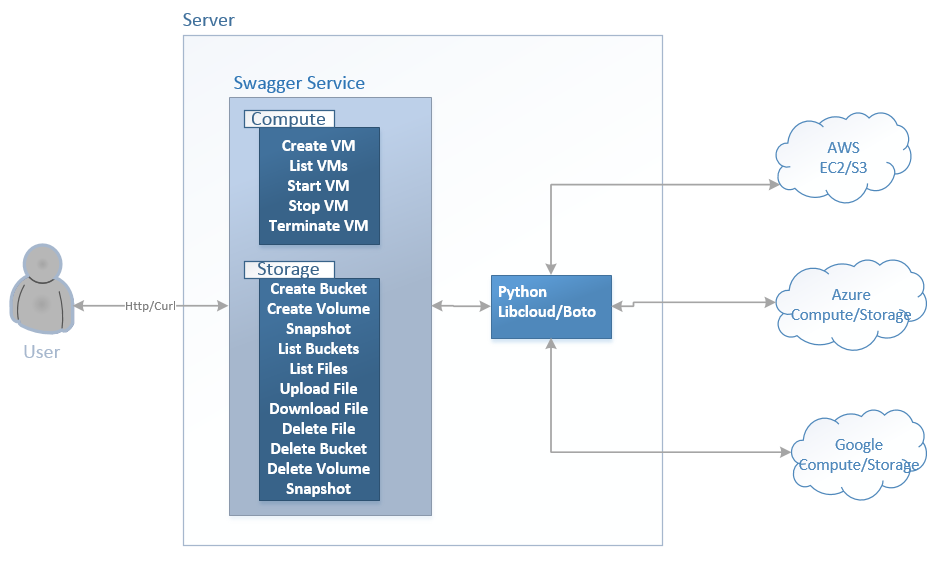
\includegraphics[width=\columnwidth]{images/proj-arch.png}
  \caption{Project Architecture}\label{F:arch}
\end{figure}

A layered approach was used so that a new implementation could be easily
integrated into the solution. Figure~\ref{f:layerd-arch} depicts the layered
approach for this service.

\begin{figure}[ht]
  \centering
  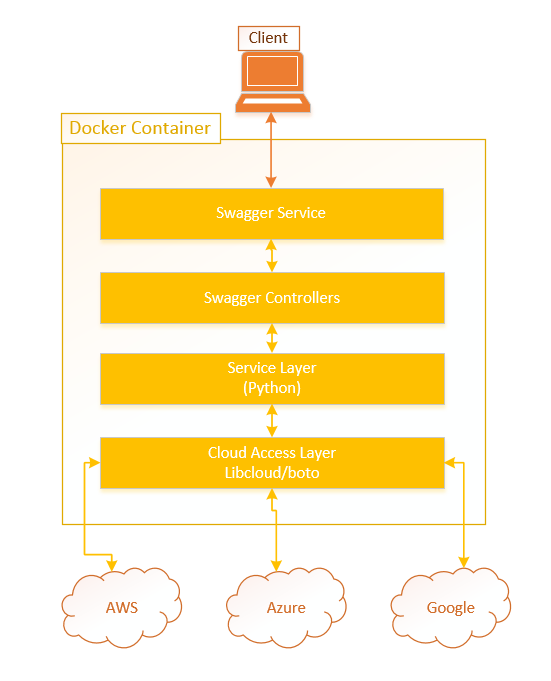
\includegraphics[width=\columnwidth]{images/layred-arch.PNG}
  \caption{Layered Architecture}\label{f:layerd-arch}
\end{figure}

\section{Other technologies used}
The other technologies leveraged for implementation are listed below. The
solution leverages these technologies yet the paper does not describe their
use in detail.

\begin{description}

\item{\bf Python.} Python was the underlying language that was used to bridge
the use of libcloud and boto into the Swagger platform. Multiple scripts were
written in python that would handle credential handling to the methods that
would interact with Compute or Storage resources. Both libcloud and boto3 are
available as native libraries for Python and it is also salient that Python was
a language of choice. Other languages do offer cloud SDKs yet they were not
explored.
\item{\bf Swagger.} Swagger and Swagger Codegen was used to generate the
documentation and design to enable a RESTful API implementation of the python
scripts. Swagger was leveraged to implement the REST interfaces to
align with course content. There are other frameworks available such as Flask
or
Django that were not assessed.
\item{\bf Amazon Web Services.} AWS natively supports boto3 which provided
robust options on what could be delivered via REST. Also, as AWS is the
industry
leader, there is significant open-source development available that provided
examples of how to use libcloud and boto3. AWS also was the most prominent when
it came to features available and features mapped into libcloud for usage.
\item{\bf Google Cloud.} GCE has an in-depth integration available with
libcloud and Apache provides very detailed examples on how to use libcloud.
Google Cloud is missing some APIs compared to AWS and as such, they are not
available for portability testing.
\item{\bf Microsoft Azure.} Azure is not natively supported by libcloud or
boto3
yet libcloud has extensive support for most of the available API calls.
Microsoft Azure has grown in market share and there is a high likelihood that
it
would be a target for porting to from an AWS developed solution.

\item{\bf R.} R was utilized to generate the box plot visualizations and
the summary statistics from benchmarking data.


\end{description}

\section{Methodology}

Python libraries exist now that help you abstract your project from  your cloud
provider. This may be important if you think you may need to use multiple cloud
providers or if you want to ensure you take steps to avoid provider lock-in.
There are multiple providers in this space and one of them is Apache
Libcloud~\cite{hid-sp18-518-LibCloud} To put it simply, this library allows you
to code simple resource  management that is independent of cloud provider
specific API calls.

Our research is intended to prove that their is significant value to leveraging
frameworks that provide portability. By comparing the native porting of an
application to a defined RESTful API, we theorize the porting of a service
between cloud providers will be more efficient. The combination of open-source
portability python libraries, the speed of Swagger, and the standardization of
REST will be a combination that will drastically improve portability.

The Cloud Security Council has broken cloud portability into five measurable
aspects of instruction, syntactic, metadata, behavior and policy. We will
leverage the instruction aspect, where the correct application instructions are
followed when ported, and the syntactic facet where porting between providers
is
transparent to the end user. This implies our testing is more closely aligned
with real-world adoption but assumes aspects like policy are left
unattended.~\cite{hid-sp18-518-Cloud-Council}

The instruction facet looks to assess whether the intended target that is being
ported to is capable of ``understanding and executing the instructions
contained
in the executable artifacts of the
application.''~\cite{hid-sp18-518-Cloud-Council} This is a strong consideration
if you are running code that depends on an underlying runtime environment,
especially if it depends on a specific environment such as the difference
between Java Runtime 7 or 8. When the porting is poorly executed, it may result
in execution failures, poor performance or even worse, the instruction appears
to run yet gives inaccurate results that must be found by regression testing.

The syntactic element looks to identify the ease of the solution to alleviate
knowledge of the underlying syntax for the cloud provider API or needing to
manually convert different unit sizes. This is salient when providers may use
custom naming conventions or if the cloud provider expects steps to be executed
in a specific fashion. This is also important at higher abstraction layers such
as the application data itself, where the ``PaaS service may provide instances
of databases ready-to-use, in which case the actual databases provided may be
sensitive to the data syntax of the customer
data.''~\cite{hid-sp18-518-Cloud-Council} The syntactic element is also where
we will highlight issues for cross-platform support in instances where the
target provider either does not have API support or libcloud does not support
yet.

To experiment, we leveraged the following resources.

\begin{itemize}

\item Swagger development to design/build API services for UI
\item Python development to leverage libcloud
\item Amazon Web Services, Azure, and Google Cloud documentation
\item Swagger API documentation
 
\end{itemize}


To reflect on the three cloud providers chosen, the results were expected to
skew towards the strengths and weaknesses of each provider. AWS is considered
the most mature provider with a very deep API offering where solutions like
Azure are making progress. Alternatively, Data Motion states ``Google developed
the Kubernetes standard that AWS and Azure now offer and GCP specializes in
high compute offerings like Big Data, analytics and machine
learning~\cite{hid-sp18-518-DataMotion}.''

\begin{figure}[!ht]
  \centering
  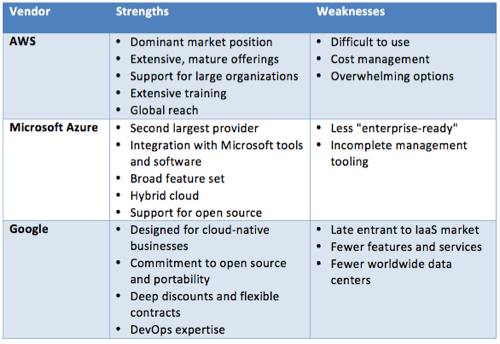
\includegraphics[width=\columnwidth]{images/aws-azure-google.png}
  \caption{Provider Comparison}\label{F:comparison}
\end{figure}

To determine the effectiveness, we have chosen to measure the cycle time on
porting a solution without libcloud to two alternatives, leveraging native
libcloud only and then our RESTful implementation of libcloud. Additionally, we
will measure the lead time metrics on using a RESTful API compared to the
command line python libraries to determine if removing the expectation for
portability can improve application development speed.

\subsection{Code Organization}

The code related to the project is organized as described in
Figure~\ref{c:code-structure}
\begin{figure}[htb]
\begin{verbatim}
code
    - Makefile
    - Dockerfile
    - compute-storage.yml
    - benchmarking.sh
    - etc
        - credentials.yml
        - google key file
    - aws
        - python scripts
   -  azure
        - python scripts
    - google
        - python scripts
\end{verbatim}
\caption{Code Structure}\label{c:code-structure}
\end{figure}

Code details
\begin{itemize}
\item \emph{Makefile} - Makefile script contains commands to
generate Swagger REST service code, import required packages,
copy files on the desired location, start Swagger service, test
Swagger service, build docker container, start and stop docker
container.
\item \emph{Dockerfile} - builds docker container
\item \emph{compute-storage.yml} - contains Swagger REST service
specification
\item \emph{etc} - this directory contains all configuration related files.
\emph{credentials.yml} file contains
authentication information required by AWS, AZURE, and Google
cloud. This directory also contains key file required by Google cloud for the
connection.
\item \emph{aws} - this directory contains Swagger controllers 
and python scripts for various operations on Amazon AWS cloud services
\item \emph{azure} - this directory contains Swagger controllers
and python scripts for various operations on Azure cloud services
\item \emph{google} - this directory contains Swagger controllers
and python scripts for various operations on Google cloud services
\item \emph{benchmarking.sh} - this script contains commands to generate data
for benchmarking
\end{itemize}

\subsection{Deployment}

The Swagger service can be deployed as docker container or
standalone service on any server type. The Makefile contains commands to 
build and run the docker container. Makefile also contains commands to build
the Swagger service and start Swagger service as a standalone application. Once
the service is deployed, it can be accessed through any browser or curl-like
utility.


\subsection{Usage}

There are certain pre-requisites for each cloud to use
this REST service.
\begin{itemize}
\item \emph{AWS} - AWS account along with access key and a secret key is
required to connect AWS cloud.
\item \emph{Azure}
Azure tenant ID, subscription ID, application id and password is required to
connect Azure cloud.
\item \emph{Google}
Google service account ID, project ID along with key file is required to
connect Google cloud.
\end{itemize}
This information should be kept confidential and need to be configured in the
yml file under the etc directory. The key file generated for Google cloud will
also need to be kept in this directory. Default VM parameters like image, size,
and region can be specified in the configuration and Swagger specification
file.

Table\ref{t:serviceFunctions} describes functions provided by the Swagger
service.
\begin{table}[htb]
\centering
\caption{Service Calls}\label{t:serviceFunctions}
\begin{tabular} {p{5cm}|p{3.5cm}}
Path & Description \\
\toprule
/compute/aws/ec2    & Creates AWS VM \\
/compute/aws/ec2/findByRegion & List AWS VMs based on region \\
/compute/aws/ec2/\{vmname\} & Get AWS VM details by VM Name \\
/compute/aws/ec2/\{vmname\}/start & Start AWS VM \\
/compute/aws/ec2/\{vmname\}/stop & Stop AWS VM \\
/compute/aws/ec2/\{vmname\}/terminate & Terminate AWS VM \\
/storage/aws/s3/bucket & List all AWS S3 buckets \\
/storage/aws/s3/bucket & Post method to create S3 bucket \\
/storage/aws/s3/bucket & Delete method to delete S3 bucket \\
/storage/aws/s3/\{bucketName\} & List all files inside the bucket \\
/storage/aws/s3/\{bucketName\}/ deleteFile & Delete file from bucket \\
/storage/aws/s3/\{bucketName\}/ uploadFile & Upload file to AWS S3 bucket \\
/storage/aws/s3/\{bucketName\}/ downloadFile & Download file from S3 to the
/download directory \\
/compute/azure/createvm & Create VM on Azure cloud \\
/compute/azure/deletevm & Delete or teminate Azure VM \\
/compute/azure/startvm & Start Azure VM \\
/compute/azure/stopvm & Stop Azure VM \\
/compute/azure/listvm & List Azure VMs \\
/storage/azure/createVol & Create Azure volume \\
/storage/azure/createVolSnap & Create Azure volume snapshot \\
/storage/azure/deleteVol & Delete Azure volume \\
/storage/azure/deleteVolSnap & Delete Azure volume snapshot \\
/compute/google/createvm & Create VM on Google cloud \\
/compute/google/deletevm & Delete or teminate Google VM \\
/compute/google/startvm & Start Google VM \\
/compute/google/stopvm & Stop Google VM \\
/compute/google/listvm & List Google VMs \\
/storage/google/createVol & Create Google volume \\
/storage/google/createVolSnap & Create Google volume snapshot \\
/storage/google/deleteVol & Delete Google volume \\
/storage/google/deleteVolSnap & Delete Google volume snapshot \\
\end{tabular}
\end{table}

\subsection{Leveraging libcloud library with Python}

To use the libcloud library in your python environment, you install the
apache-libcloud package using the Python package management system, pip.
Libcloud currently supports Python versions 2.5, 2.6, 2.7 and Python 3. To use
libcloud as a library, leverage Python and import libcloud like any other
library. A useful feature to use in Python is the help function which will
provide you a simple manual on further use of libcloud.

As an example, we leveraged libcloud to configure and manage EC2 in AWS. We
first needed to configure credentials for an active cloud provider account and
then configured libcloud provider to use that account. To be able to access AWS
S3 from libcloud, we need the access key to be specified in the call. An access
key can be setup on AWS console by navigating to My Security credentials,
Encryption Keys, and then Access Keys.Next, local variables were defined to
store the credentials to be used. Once that was set up, we defined the EC2 
driver with our region preference, which was AWS us-east-1, the most full
featured region. This is because there are additional tasks that must be taken
with SSH keys. We used our browser to review EC2 and finalize the setup.

A Python example for leveraging libcloud to list available containers in an AWS
S3 instance is shown below. The key steps are importing the libraries and
leveraging the functions that enable connectivity, authentication and
authorization. Once that is complete, you can pull or push information using
the family of functions that are available in Libcloud for your flavor of cloud
provider, in this instance which is AWS.

\begin{figure}[htb]

\begin{verbatim}

from libcloud.storage.types import Provider
from libcloud.storage.providers import get_driver


cls = get_driver(Provider.S3_US_EAST2)
driver = cls('api key', 'api secret key')

d = driver.list_containers();

print d;

\end{verbatim}

\caption{Leveraging Libcloud
~\cite{hid-sp18-518-LibCloud}}\label{c:libcloud-example}

\end{figure}

The following table\ref{t:libcloudtable} is a breakdown of other functions
that were leveraged in
Libcloud during our development. The list is tailored towards only what we used
directly. If a feature is specific towards a certain cloud provider, as in it
was not completely abstracted by Libcloud, the description will point out the
customized use.

\begin{table}[htb]
\centering
\caption{LibCloud features leveraged}\label{t:libcloudtable}
\begin{tabular} {p{2.5cm}|p{5cm}}
Command & Description\\
\toprule
\verb|get_driver()| & How to choose the primary cloud provider that will be
used by following functions. We leveraged Amazon Web Services, Microsoft Azure
and Google Cloud as targets for this method.\\
\verb|dns()| & Used to configure DNS for compute resources. This is an example
of a
late-stage call to further define how a virtual machine should be configured.\\

\verb|get_driver_lb()| & Used to configure load balancing for compute
resources. This
field is a great example of the power of cloud computing and RESTful API as
redundant, highly available virtual machines can be built quickly and if you
choose, by default.\\

\verb|list_nodes()| & Used to enumerate the nodes already created within the
cloud
provider. This call can be automated to routinely audit usage of virtual
machines to identify trends for usage.\\

\verb|list_sizes()| & Used to enumerate the size of the VM and supporting
components.
This method is commonly used to reduce costs and identify VMs that may have
grown beyond a comfortable level.\\

\verb|list_images()| & Used to enumerate the avaiable, deployable images the
cloud
provider makes available. This parameter is typically used before a call to
generate a virtual machine to ensure the image is still provided by the cloud
provider.\\

\verb|get_image()| & Used to pull the unique identifier for the human-readable
name
for the chosen image\\

\verb|ex_get_node()| & Used to pull the unique identifier for one or many
VMs.\\

\verb|create_node()| & Used in conjuection with image listing to deploy a new
VM.\\

\verb|ex_start_node()| & Used to tell a previously built VM to boot.\\

\verb|ex_stop_node()| & Used to direct a VM to begin shutdown gracefully.\\

\verb|destroy_node()| & Used to delete a VM and will return success. This
method is
one where human error can lead to significant damages and leveraging REST, the
solution can confirm deletion with a user or restrict deletion. It also can
simply ensure virtual machines actually are deleted after a certain threshold
as
it is common for human-generated virtual machines to be left running that leads
to unwarranted costs.\\

\verb|ex_get_volume()| & Used to enumerate the unique identifier for cloud
storage
typically used by a VM.\\

\verb|create_volume()| & Used to add addtional storage to a VM.\\

\verb|destroy_volume()| & Used to delete storage or snapshot to recover
storage space.\\
\end{tabular}
\end{table}

\subsection{Leveraging boto3 library with Python}

In order to leverage boto3 within a python console, you simply can install
using
pip like we have done with libcloud. Boto3 was developed with Python 3 in mind
yet backwards compatibility is available to Python 2.7 and 2.6.5. A salient
point to stress is that boto3 is different than boto, like how Python 2 is
different than Python 3. The authors of boto stress that boto3 should be used
as
boto is only supported for older implementations. The features are similar yet
boto will eventually be deprecated and developers will have to migrate to
boto3.~\cite{hid-sp18-518-AWS-boto3}

As with all interactions with cloud providers, the aspect of credentials and
privileges must be addressed before successful use of the libraries. Since
boto3
powers the use of the AWS CLI, we found the use of the AWS CLI to be the most
effective way to configure credentials. The credential space is shared between
boto3 and AWS CLI and there is less error when using the user-friendly AWS CLI.
Credentials can be hardcoded as well and examples are provided by
Amazon.~\cite{hid-sp18-518-Boto3} The last step that must be taken is define
the
location you wish boto3 to focus on such as AWS regions. Multi-region support
is
limited and if you do not define an alternate region, it will use us-east-1.

Below is an example of how we leveraged boto3 to start and stop an instance
defined in AWS EC2. The python script is passed two parameters, On or Off, and
the instance ID you wish to change. The parameters are ultimately passed to
boto3 to connect to your EC2 instances and perform the action.

\begin{figure}[htb]
\begin{verbatim}

# To start the instance
$ python boto_ec2.py <on> <instance id>

# To stop the instance
$ python boto_ec2.py <off> <instance id>

# Add below code to a file named boto_ec2.py
# 
# # # # # # # # # # # # # # # # # # # # # # # # # # # # # # # 
import boto3

action = sys.argv[1].upper()

ec2 = boto3.client('ec2')

\end{verbatim}

\caption{Leveraging Boto3~\cite{hid-sp18-518-Boto3}}\label{c:boto3-example}

\end{figure}

Once boto3 is imported, the object ec2 is leveraged for ease of use. The client
method is defined with the intended cloud provider environment, in this case it
is AWS EC2. The calls in Python using the variable are then vendor agnostic.
For
the methods for starting and stopping instances, boto3 allows the author to
follow a common syntax structure that will map the parameters into the
underlying vendor API calls. Last, boto3 will capture the returned output
provided by the vendor and will make it available for your use. In this python
script, we have captured the response into a variable for later use and to show
that it works as defined, the output is sent to the console.

\section{Use Case: Rest API calls}

The final outcome of the code development was an ability to leverage an HTTP
call to request usage of cloud services. For example, below is a sample of an
API call where elements are passed with POST to provide the parameters needed
for libcloud or boto to initiate the call. When the call is completed, the API
returns a string on what was requests. The parameters are sent in JSON format
and are extensible into other platforms. Some feature enhancements for the REST
API call would be error handling if libcloud or boto have issues executing the
call.  

Using a utility like curl, you can push a JSON blob using POST. The RESTful API
is organized into folders, for example, where computer resources are under a
URI
structure prefaced with the intended use, like compute, and then the cloud
provider you wish to use, like ec2. The JSON blob contains the parameters that
will be in the body of the POST that will be used by Python and follows normal
HTTP syntax.

By leveraging an HTTP call allows, we have created an opportunity to extend the
solution for automation or to provide a browser-based user experience. Both of
those types of solutions would improve the scalability of what can be done
compared to cloud provider UI or the provided command-line tools. Both
solutions
are also less prone to error by incorrect data entry or mistakes by overly
broad
permissions. 

The use of Swagger has also helped define the RESTful API into a well-known
standard. The markup file for the solution contains the documentation for use
and defines what type of field is expected, from strings to integers. The
benefit from Swagger is that a very thorough explanation of how to use the API
is provided and the efforts to generate the documentation is very light.
Additionally, it is automated and the accuracy is complete compared to a manual
effort to capture how to use the RESTful API to call libcloud or boto3.

The API call maps to the following Python script which would build a virtual
machine. The method requires multiple parameters that are mapped into the
RESTful API calls. The JSON blob would pass the paramenters into the Python
script to leverage the \verb|get\_image| and \verb|create\_node| features in
libcloud.

\begin{figure}[htb]
\begin{verbatim}
def
createAzureVM(vmname,vmsize,image_name,resource_group,storage_account,nw_intf,
blob_container): 

#print region
#
	urn='Canonical:UbuntuServer:16.04-LTS:latest'

	image=driver.get_image(urn, location=None)

	print image
	
\end{verbatim}

\caption{Python script example}\label{c:Python-example}
\end{figure}	

The error handling by the script provides the user feedback on what happened
and how to resolve. A future enhancement would be to map the method return back
to the RESTful API and the error could be presented to the user in the user
interface they are using to leverage the API. When the method works correctly,
the parameters passed into the method could be leveraged to confirm the correct
virtual machine was created and also used to enhance the message sent back to
the user.

\section{Benchmarking}

A benchmarking shell script is provided that tests the timing performance
between the cloud providers when leveraging libcloud. The script would initiate
the measurement when the API call is made and then consider the request
complete when libcloud interprets the cloud provider response and returns it.
For the benchmarking, a series of ten tests were performed per method per the
three cloud providers. The output for the benchmarks were captured for later
visualizations to interpret how well libcloud works for different types of
requests and for different providers. All three providers successfully
generated virtual machines, as expected, with the parameters provided.
Additionally, libcloud abstracted the syntax successfully for all three
providers. Table\ref{t:benchmarking} shows the benchmarking test results.

\begin{table}[htb]
\centering
\caption{Benchmarking Test Results}\label{t:benchmarking}
\begin{tabular} {p{3cm}|p{3cm}|p{5cm}|p{3cm}}
Cloud Provider & Type & Operation Name & Duration (secs) \\
\toprule
AWS & Compute & Create VM & 75 \\
AWS & Compute & List VM & 179 \\
AWS & Compute & Get VM Details & 5 \\
AWS & Compute & Stop VM & 13  \\
AWS & Compute & Start VM & 5  \\
AWS & Compute & Delete VM & 7  \\
AWS & Storage & Get Vol/Bucket Details & 0  \\
AWS & Storage & Create Vol/Bucket & 1  \\
AWS & Storage & Upload File to S3 & 0  \\
AWS & Storage & List Vol/Bucket Details & 1  \\
AWS & Storage & Download File from S3 & 0  \\
AWS & Storage & Delete S3 File & 1  \\
AWS & Storage & Delete Vol/Bucket & 1  \\
AWS & Compute & Create VM & 33  \\
AWS & Compute & List VM & 47  \\
AWS & Compute & Get VM Details & 11  \\
AWS & Compute & Stop VM & 159  \\
AWS & Compute & Start VM & 4  \\
AWS & Compute & Delete VM & 14  \\
AWS & Storage & Get Vol/Bucket Details & 3  \\
AWS & Storage & Create Vol/Bucket & 7  \\
AWS & Storage & Upload File to S3 & 1  \\
AWS & Storage & List Vol/Bucket Details & 0  \\
AWS & Storage & Download File from S3 & 1  \\
AWS & Storage & Delete S3 File & 0  \\
AWS & Storage & Delete Vol/Bucket & 1  \\
AWS & Compute & Create VM & 40  \\
AWS & Compute & List VM & 2  \\
AWS & Compute & Get VM Details & 56  \\
AWS & Compute & Stop VM & 40  \\
AWS & Compute & Start VM & 148  \\
AWS & Compute & Delete VM & 5  \\
AWS & Storage & Get Vol/Bucket Details & 12  \\
AWS & Storage & Create Vol/Bucket & 5  \\
AWS & Storage & Upload File to S3 & 6  \\
AWS & Storage & List Vol/Bucket Details & 0  \\
AWS & Storage & Download File from S3 & 1  \\
AWS & Storage & Delete S3 File & 0  \\
AWS & Storage & Delete Vol/Bucket & 1  \\
AWS & Compute & Create VM & 30  \\
AWS & Compute & List VM & 0  \\
AWS & Compute & Get VM Details & 1  \\
AWS & Compute & Stop VM & 1  \\
AWS & Compute & Start VM & 1  \\
AWS & Compute & Delete VM & 0  \\
AWS & Storage & Get Vol/Bucket Details & 1  \\
AWS & Storage & Create Vol/Bucket & 0  \\
AWS & Storage & Upload File to S3 & 1  \\
AWS & Storage & List Vol/Bucket Details & 0  \\
AWS & Storage & Download File from S3 & 1  \\
AWS & Storage & Delete S3 File & 0  \\
AWS & Storage & Delete Vol/Bucket & 1  \\
AWS & Compute & Create VM & 32  \\
AWS & Compute & List VM & 0  \\
AWS & Compute & Get VM Details & 1  \\
AWS & Compute & Stop VM & 1  \\
AWS & Compute & Start VM & 1  \\
AWS & Compute & Delete VM & 1  \\
AWS & Storage & Get Vol/Bucket Details & 0  \\
AWS & Storage & Create Vol/Bucket & 1  \\
AWS & Storage & Upload File to S3 & 0  \\
AWS & Storage & List Vol/Bucket Details & 1  \\
AWS & Storage & Download File from S3 & 0  \\
AWS & Storage & Delete S3 File & 0  \\
AWS & Storage & Delete Vol/Bucket & 1  \\
AWS & Compute & Create VM & 33  \\
AWS & Compute & List VM & 1  \\
AWS & Compute & Get VM Details & 0  \\
AWS & Compute & Stop VM & 1  \\
AWS & Compute & Start VM & 1  \\
AWS & Compute & Delete VM & 1  \\
AWS & Storage & Get Vol/Bucket Details & 0  \\
AWS & Storage & Create Vol/Bucket & 1  \\
AWS & Storage & Upload File to S3 & 1  \\
AWS & Storage & List Vol/Bucket Details & 0  \\
AWS & Storage & Download File from S3 & 0  \\
AWS & Storage & Delete S3 File & 1  \\
AWS & Storage & Delete Vol/Bucket & 0  \\
AWS & Compute & Create VM & 35  \\
AWS & Compute & List VM & 1  \\
AWS & Compute & Get VM Details & 1  \\
AWS & Compute & Stop VM & 1  \\
AWS & Compute & Start VM & 1  \\
AWS & Compute & Delete VM & 1  \\
AWS & Storage & Get Vol/Bucket Details & 0  \\
AWS & Storage & Create Vol/Bucket & 1  \\
AWS & Storage & Upload File to S3 & 1  \\
AWS & Storage & List Vol/Bucket Details & 0  \\
AWS & Storage & Download File from S3 & 1  \\
AWS & Storage & Delete S3 File & 0  \\
AWS & Storage & Delete Vol/Bucket & 1  \\
AWS & Compute & Create VM & 33  \\
AWS & Compute & List VM & 1  \\
AWS & Compute & Get VM Details & 1  \\
AWS & Compute & Stop VM & 1  \\
AWS & Compute & Start VM & 1  \\
AWS & Compute & Delete VM & 1  \\
AWS & Storage & Get Vol/Bucket Details & 2  \\
AWS & Storage & Create Vol/Bucket & 0  \\
AWS & Storage & Upload File to S3 & 1  \\
AWS & Storage & List Vol/Bucket Details & 0  \\
AWS & Storage & Download File from S3 & 1  \\
AWS & Storage & Delete S3 File & 0  \\
AWS & Storage & Delete Vol/Bucket & 1  \\
AWS & Compute & Create VM & 34  \\
AWS & Compute & List VM & 0  \\
AWS & Compute & Get VM Details & 1  \\
AWS & Compute & Stop VM & 1  \\
AWS & Compute & Start VM & 1  \\
AWS & Compute & Delete VM & 1  \\
AWS & Storage & Get Vol/Bucket Details & 0  \\
AWS & Storage & Create Vol/Bucket & 1  \\
AWS & Storage & Upload File to S3 & 0  \\
AWS & Storage & List Vol/Bucket Details & 1  \\
AWS & Storage & Download File from S3 & 0  \\
AWS & Storage & Delete S3 File & 1  \\
AWS & Storage & Delete Vol/Bucket & 0  \\
AWS & Compute & Create VM & 31  \\
AWS & Compute & List VM & 0  \\
AWS & Compute & Get VM Details & 1  \\
AWS & Compute & Stop VM & 1  \\
AWS & Compute & Start VM & 1  \\
AWS & Compute & Delete VM & 1  \\
AWS & Storage & Get Vol/Bucket Details & 0  \\
AWS & Storage & Create Vol/Bucket & 1  \\
AWS & Storage & Upload File to S3 & 0  \\
AWS & Storage & List Vol/Bucket Details & 1  \\
AWS & Storage & Download File from S3 & 0  \\
AWS & Storage & Delete S3 File & 1  \\
AWS & Storage & Delete Vol/Bucket & 0  \\
Google & Compute & Create VM & 11  \\
Google & Compute & List VM & 1  \\
Google & Compute & Stop VM & 163  \\
Google & Compute & Start VM & 13  \\
Google & Compute & Delete VM & 154  \\
Google & Storage & Create Vol/Bucket & 6  \\
Google & Storage & Create Volume Snapshot & 32  \\
Google & Storage & Delete Volume Snapshot & 89  \\
Google & Storage & Delete Vol/Bucket & 7  \\
Google & Compute & Create VM & 12  \\
Google & Compute & List VM & 5  \\
Google & Compute & Stop VM & 43  \\
Google & Compute & Start VM & 21  \\
Google & Compute & Delete VM & 70  \\
Google & Storage & Create Vol/Bucket & 189  \\
Google & Storage & Create Volume Snapshot & 13  \\
Google & Storage & Delete Volume Snapshot & 4  \\
Google & Storage & Delete Vol/Bucket & 6  \\
Google & Compute & Create VM & 24  \\
Google & Compute & List VM & 5  \\
Google & Compute & Stop VM & 60  \\
Google & Compute & Start VM & 9  \\
Google & Compute & Delete VM & 58  \\
Google & Storage & Create Vol/Bucket & 158  \\
Google & Storage & Create Volume Snapshot & 126  \\
Google & Storage & Delete Volume Snapshot & 118  \\
Google & Storage & Delete Vol/Bucket & 8  \\
Google & Compute & Create VM & 11  \\
Google & Compute & List VM & 6  \\
Google & Compute & Stop VM & 52  \\
Google & Compute & Start VM & 22  \\
Google & Compute & Delete VM & 46  \\
Google & Storage & Create Vol/Bucket & 218  \\
Google & Storage & Create Volume Snapshot & 13  \\
Google & Storage & Delete Volume Snapshot & 4  \\
Google & Storage & Delete Vol/Bucket & 6  \\
Google & Compute & Create VM & 11  \\
Google & Compute & List VM & 5  \\
Google & Compute & Stop VM & 54  \\
Google & Compute & Start VM & 21  \\
Google & Compute & Delete VM & 53  \\
Google & Storage & Create Vol/Bucket & 179  \\
Google & Storage & Create Volume Snapshot & 14  \\
Google & Storage & Delete Volume Snapshot & 3  \\
Google & Storage & Delete Vol/Bucket & 6  \\
Google & Compute & Create VM & 11  \\
Google & Compute & List VM & 5  \\
Google & Compute & Stop VM & 59  \\
Google & Compute & Start VM & 20  \\
Google & Compute & Delete VM & 53  \\
Google & Storage & Create Vol/Bucket & 180  \\
Google & Storage & Create Volume Snapshot & 12  \\
Google & Storage & Delete Volume Snapshot & 3  \\
Google & Storage & Delete Vol/Bucket & 6  \\
Google & Compute & Create VM & 9  \\
Google & Compute & List VM & 5  \\
Google & Compute & Stop VM & 45  \\
Google & Compute & Start VM & 21  \\
Google & Compute & Delete VM & 54  \\
Google & Storage & Create Vol/Bucket & 180  \\
Google & Storage & Create Volume Snapshot & 10  \\
Google & Storage & Delete Volume Snapshot & 4  \\
Google & Storage & Delete Vol/Bucket & 6  \\
Google & Compute & Create VM & 11  \\
Google & Compute & List VM & 5  \\
Google & Compute & Stop VM & 46  \\
Google & Compute & Start VM & 57  \\
Google & Compute & Delete VM & 76  \\
Google & Storage & Create Vol/Bucket & 147  \\
Google & Storage & Create Volume Snapshot & 14  \\
Google & Storage & Delete Volume Snapshot & 5  \\
Google & Storage & Delete Vol/Bucket & 7  \\
Google & Compute & Create VM & 9  \\
Google & Compute & List VM & 30  \\
Google & Compute & Stop VM & 45  \\
Google & Compute & Start VM & 11  \\
Google & Compute & Delete VM & 158  \\
Google & Storage & Create Vol/Bucket & 5  \\
Google & Storage & Create Volume Snapshot & 14  \\
Google & Storage & Delete Volume Snapshot & 4  \\
Google & Storage & Delete Vol/Bucket & 7  \\
Google & Compute & Create VM & 15  \\
Google & Compute & List VM & 29  \\
Google & Compute & Stop VM & 57  \\
Google & Compute & Start VM & 39  \\
Google & Compute & Delete VM & 148  \\
Google & Storage & Create Vol/Bucket & 5  \\
Google & Storage & Create Volume Snapshot & 13  \\
Google & Storage & Delete Volume Snapshot & 4  \\
Google & Storage & Delete Vol/Bucket & 7  \\
Azure & Compute & Create VM & 5  \\
Azure & Compute & List VM & 1  \\
Azure & Compute & Stop VM & 13  \\
Azure & Compute & Start VM & 23  \\
Azure & Compute & Delete VM & 178  \\
Azure & Storage & Create Vol/Bucket & 3  \\
Azure & Storage & Create Volume Snapshot & 1  \\
Azure & Storage & Delete Volume Snapshot & 0  \\
Azure & Storage & Delete Vol/Bucket & 0  \\
Azure & Compute & Create VM & 6  \\
Azure & Compute & List VM & 1  \\
Azure & Compute & Stop VM & 13  \\
Azure & Compute & Start VM & 24  \\
Azure & Compute & Delete VM & 177  \\
Azure & Storage & Create Vol/Bucket & 1  \\
Azure & Storage & Create Volume Snapshot & 0  \\
Azure & Storage & Delete Volume Snapshot & 1  \\
Azure & Storage & Delete Vol/Bucket & 0  \\
Azure & Compute & Create VM & 147  \\
Azure & Compute & List VM & 10  \\
Azure & Compute & Stop VM & 154  \\
Azure & Compute & Start VM & 24  \\
Azure & Compute & Delete VM & 97  \\
Azure & Storage & Create Vol/Bucket & 5  \\
Azure & Storage & Create Volume Snapshot & 6  \\
Azure & Storage & Delete Volume Snapshot & 0  \\
Azure & Storage & Delete Vol/Bucket & 0  \\
Azure & Compute & Create VM & 16  \\
Azure & Compute & List VM & 2  \\
Azure & Compute & Stop VM & 54  \\
Azure & Compute & Start VM & 24  \\
Azure & Compute & Delete VM & 240  \\
Azure & Storage & Create Vol/Bucket & 5  \\
Azure & Storage & Create Volume Snapshot & 13  \\
Azure & Storage & Delete Volume Snapshot & 4  \\
Azure & Storage & Delete Vol/Bucket & 6  \\
Azure & Compute & Create VM & 27  \\
Azure & Compute & List VM & 1  \\
Azure & Compute & Stop VM & 61  \\
Azure & Compute & Start VM & 21  \\
Azure & Compute & Delete VM & 199  \\
Azure & Storage & Create Vol/Bucket & 117  \\
Azure & Storage & Create Volume Snapshot & 128  \\
Azure & Storage & Delete Volume Snapshot & 5  \\
Azure & Storage & Delete Vol/Bucket & 6  \\
Azure & Compute & Create VM & 16  \\
Azure & Compute & List VM & 2  \\
Azure & Compute & Stop VM & 64  \\
Azure & Compute & Start VM & 21  \\
Azure & Compute & Delete VM & 248  \\
Azure & Storage & Create Vol/Bucket & 5  \\
Azure & Storage & Create Volume Snapshot & 12  \\
Azure & Storage & Delete Volume Snapshot & 4  \\
Azure & Storage & Delete Vol/Bucket & 6  \\
Azure & Compute & Create VM & 15  \\
Azure & Compute & List VM & 2  \\
Azure & Compute & Stop VM & 66  \\
Azure & Compute & Start VM & 21  \\
Azure & Compute & Delete VM & 216  \\
Azure & Storage & Create Vol/Bucket & 4  \\
Azure & Storage & Create Volume Snapshot & 13  \\
Azure & Storage & Delete Volume Snapshot & 3  \\
Azure & Storage & Delete Vol/Bucket & 6  \\
Azure & Compute & Create VM & 15  \\
Azure & Compute & List VM & 2  \\
Azure & Compute & Stop VM & 70  \\
Azure & Compute & Start VM & 21  \\
Azure & Compute & Delete VM & 217  \\
Azure & Storage & Create Vol/Bucket & 5  \\
Azure & Storage & Create Volume Snapshot & 10  \\
Azure & Storage & Delete Volume Snapshot & 3  \\
Azure & Storage & Delete Vol/Bucket & 6  \\
Azure & Compute & Create VM & 13  \\
Azure & Compute & List VM & 2  \\
Azure & Compute & Stop VM & 57  \\
Azure & Compute & Start VM & 24  \\
Azure & Compute & Delete VM & 214  \\
Azure & Storage & Create Vol/Bucket & 4  \\
Azure & Storage & Create Volume Snapshot & 11  \\
Azure & Storage & Delete Volume Snapshot & 3  \\
Azure & Storage & Delete Vol/Bucket & 6  \\
Azure & Compute & Create VM & 15  \\
Azure & Compute & List VM & 2  \\
Azure & Compute & Stop VM & 57  \\
Azure & Compute & Start VM & 57  \\
Azure & Compute & Delete VM & 207  \\
Azure & Storage & Create Vol/Bucket & 5  \\
Azure & Storage & Create Volume Snapshot & 13  \\
Azure & Storage & Delete Volume Snapshot & 5  \\
Azure & Storage & Delete Vol/Bucket & 7  \\
\end{tabular}
\end{table}



\subsection{Virtual Machine - Start}

It was also observed that all three providers were able to execute successfully
across all 10 tests. AWS was benchmarked as the leader of the three with an
average execution time of 16.4 seconds. AWS was surprisingly able to still be
the leader on average with a significant outlier in the dataset where one test
took 148 seconds to complete. The other two providers, Google and
Azure, started up in 23.4s and 26s respectively. Out of the five benchmarks,
starting a virtual machine when using libcloud was one of two metrics that had
two providers average within a reasonable range of each other. Figure \ref{F:vm-start}
shows the details.

\begin{figure}[!ht]
  \centering
  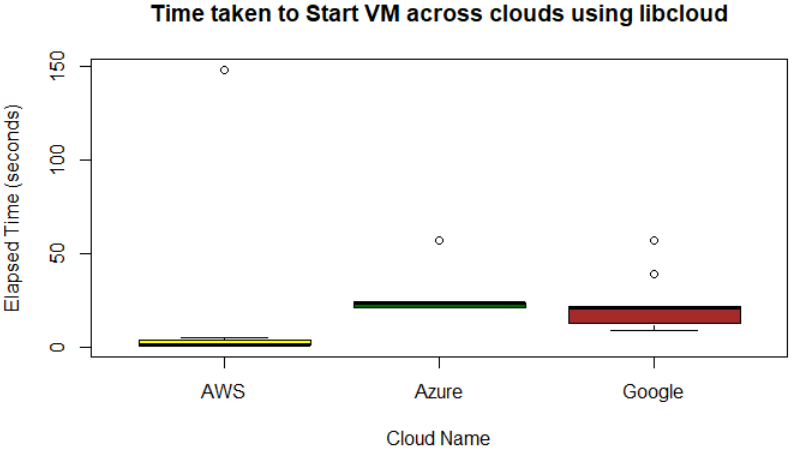
\includegraphics[width=\columnwidth]{images/StartVM.png}
  \caption{VM starting benchmark}\label{F:vm-start}
\end{figure}

\subsection{Virtual Machine - Stop}

For the stopping of virtual machines, AWS again was the clear leader in
performance. Libcloud, on average, reported a successful stop of a virtual
machine in 21.9s. For Azure, the average result was 60.9s which was marginally
better than the average for Google of 62.4s. Similar to the starting of virtual
machines, there was a clear leader and the other two providers compared evenly
with each other. The same can bee seen in figure \ref{F:vm-stop}.

\begin{figure}[!ht]
  \centering
  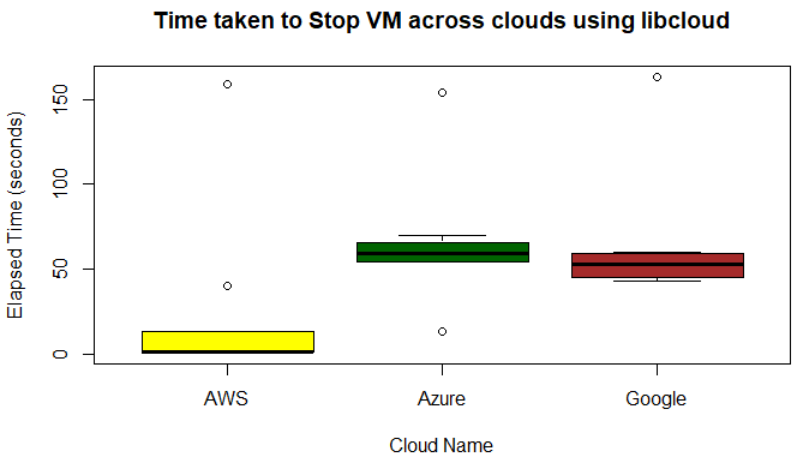
\includegraphics[width=\columnwidth]{images/StopVM.png}
  \caption{VM stopping benchmark}\label{F:vm-stop}
\end{figure}

\subsection{Virtual Machine - Create}

As you can see from figure \ref{F:vm-create} that creation of virtual machines
is where a new leader is presented with 
Google. This was expected as marketing for Google implies they are very
efficient at horizontal scaling and rapid deployment of net new virtual
machines and containers. Google was found to be able to generate a new virtual
machine in 12.4s, which is half the time it takes compared to 27.5s from Azure.
AWS trailed both with an average creation time of 37.6 seconds.

\begin{figure}[!ht]
  \centering
  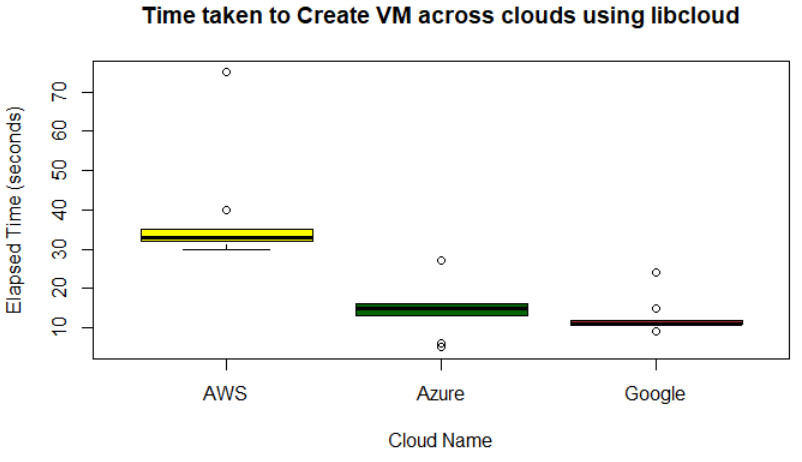
\includegraphics[width=\columnwidth]{images/CreateVM.png}
  \caption{VM creation benchmark}\label{F:vm-create}
\end{figure}

\subsection{Storage - Create}

For the creation of storage, AWS was significantly faster than the other two
providers. AWS was able to create a 1 GB volume and return success within 1.8s.
Azure was slower at 15.4s yet Google was markedly much slower with an average
speed of 126.7. Where Google was the fastest solution to create a new virtual
machine, the ability to rapidly deploy additional storage was found to be a
weakness of the Google cloud provider. We do not perceive it to be an issue
with how Libcloud requests storage from Google and it is attributed to Google
directly. The visualization of the same can be seen in Figure \ref{F:vm-volume}. 

\begin{figure}[!ht]
  \centering
  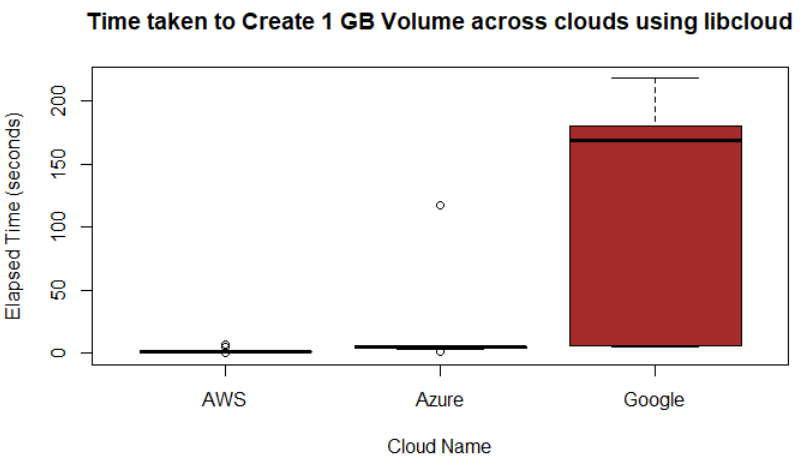
\includegraphics[width=\columnwidth]{images/Create1GBVol.png}
  \caption{Volume creation benchmark}\label{F:vm-volume}
\end{figure}

\subsection{Virtual Machine - Delete}

For the rapid decommissioning or clean up of virtual machines, AWS was also
found to be remarkably fast. Libcloud had success with all three vendors with
AWS on average reporting a virtual machine had been deleted in 3.2s. Google
came in next with an average of 87s and Azure was the slowest at
199.3s. Figure \ref{F:vm-delete} shows the details of the benchmark.



\begin{figure}[!ht]
  \centering
  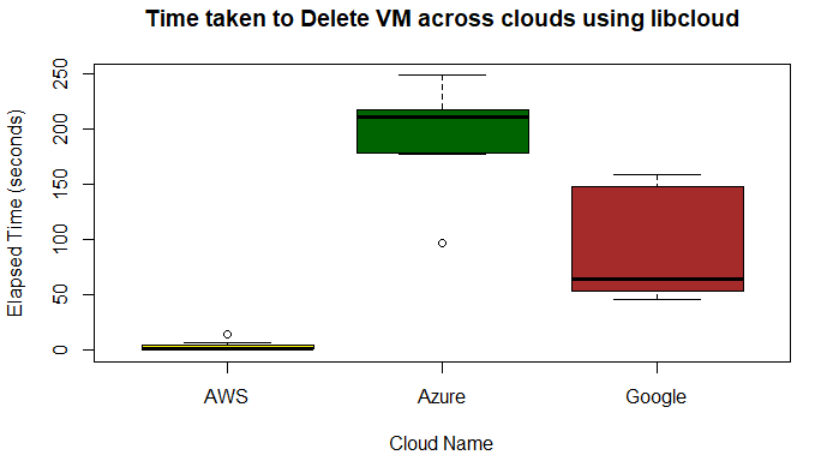
\includegraphics[width=\columnwidth]{images/DeleteVM.png}
  \caption{VM deletion benchmark}\label{F:vm-delete}
\end{figure}

\section{Results}
We had success leveraging libcloud to generate and control the execution of
cloud resources with Amazon Web Services and Microsoft Azure. We were able to
abstract away from native API calls for a cloud provider. Additionally, we were
able to map the Python scripts leveraging libcloud into RESTful APIs that were
well-documented leveraging Swagger. The solutions combined to provide a
solution that hides the intricacies of knowing how to use each vendor's API and
the verbiage they use to explain different types of cloud resources. 

While libcloud works well with all the three vendors Amazon, Microsoft and
Google,
there are certain functions that are available only for AWS such as uploading
a file or downloading a file. Libcloud integration with Google is
straightforward
and the API functions operate over string parameters whereas for Azure a Node
object has to be passed and returned in most cases. Implementation with Azure
especially required the use of a hidden or internal function usage in one of
the
cases. Due to this constraint, time to integrate Azure was significantly higher
as compared
to AWS or Google.

The use of boto3 became challenging in relation to Google Cloud. In concurrency
with what the technology review stressed, the
use of proprietary utilities like
gsutil limited what we can develop. Boto3 development was successful with AWS
resources yet at boto3 is the underlying technology for AWS utilities, the
value-add was limited to converting boto3 calls for AWS into a RESTful API.

\section{Conclusion}

Libraries available for abstracting the cloud provider from your code
development were found to be effective. The solutions are syntactically and
instructionally accurate. The solutions also had negligible impact on
performance and were easy to extend for custom usage, such as benchmarking.
The cloud providers were found to be distinct, even with an abstraction layer
such as libcloud and boto3. There were challenges with authorization and object
handling between providers that had to be handled independently. 

The project exhibited that it is possible to ensure your application could be
ported yet with significant work. Further research would be necessary to see if
a manual port of native use of cloud provider APIs is more intensive than
leveraging something like libcloud. Our perception is that efforts to ensure
portability are incomplete and if the three primary providers could incur cost
beyond API calls, there is still significant work to be done to align with the
NIST guidance of ensuring portability to get beyond where ``consumers must seek
to understand cloud services through a customized and product specific view
presented by each service provider~\cite{hid-sp18-518-NIST-293}.''

\section{Artifacts}

Code is checked-in in Github at location
\emph{https://github.com/cloudmesh-community/hid-sp18-518/tree/master/project-
code}

\begin{acks}

  The authors would like to thank Dr.~Gregor~von~Laszewski for his
  support and suggestions to write this paper.

\end{acks}

\bibliographystyle{ACM-Reference-Format}
\bibliography{report} 

\section{Work Contributions}
\begin{itemize}
\item
AWS Compute and Storage coding by Sushant Athaley
\item
Azure Compute and Storage Coding by Harshad Pitkar
\item
Google libcloud research by Michael Robinson
\item
Google Compute coding by Harshad Pitkar
\item
Google Storage Coding by Sushant Athaley
\item
Dockerfile by Sushant Athaley
\item
Makefile by Sushant Athaley
\item
Architecture explanation by Michael Robinson
\item
Architecture diagrams by Sushant Athaley
\item
Benchmarking script by Harshad Pitkar
\item
Bencmarking plots by Harshad Pitkar
\item
Benchmarking explanation by Michael Robinson
\item
Code packaging and management by Sushant Athaley
\item
Code explanation by Michael Robinson
\item
Swagger Spec by Sushant Athaley and Harshad Pitkar
\item
Service Testing by Sushant Athaley and Harshad Pitkar
\item
Code Merging by Sushant Athaley and Harshad Pitkar
\item
Project Paper by Michael Robinson and Sushant Athaley and Harshad Pitkar
\end{itemize}


